\documentclass{article}
\usepackage[margin=0.8cm]{geometry}
\usepackage{tikz}
\usetikzlibrary{arrows.meta,positioning,shapes.geometric,calc,fit,backgrounds}

\pagestyle{empty}

% Target column width for IEEE two-column layout (~8.5 cm)
\newcommand{\colw}{8.5cm}

\begin{document}

%% ════════════════════════════════════════════════════════════════════════
%%  FIGURE 1 — Offline Model Development Pipeline (PC side)
%% ════════════════════════════════════════════════════════════════════════
\noindent\resizebox{\colw}{!}{%
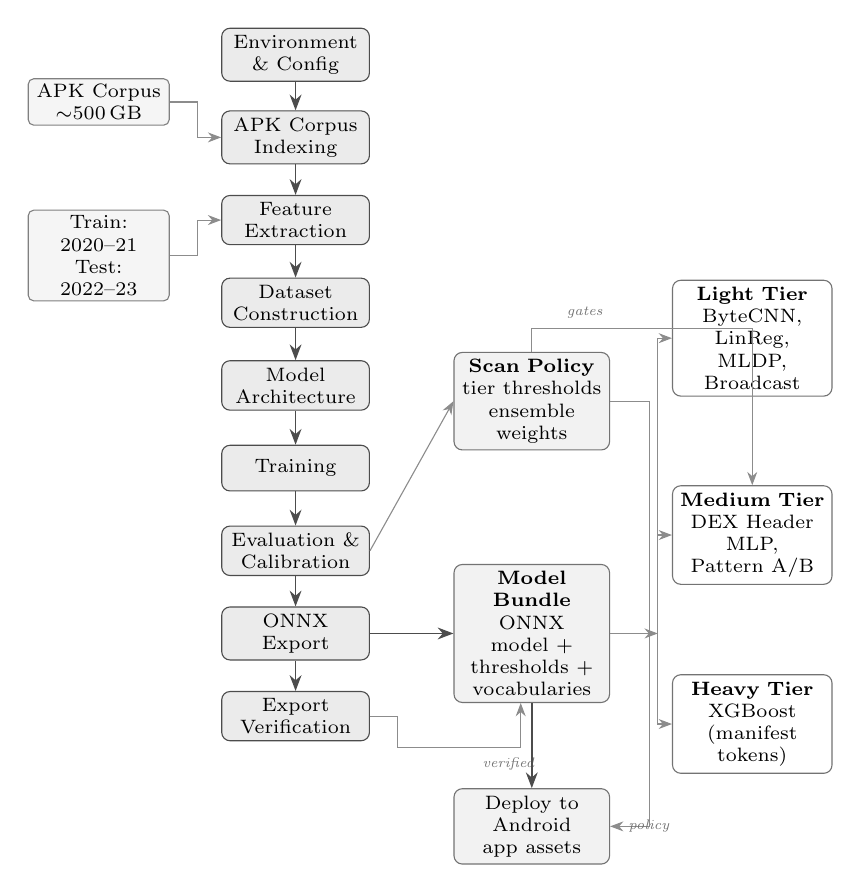
\begin{tikzpicture}[
  font=\scriptsize,
  >=Stealth,
  phase/.style={
    rectangle, rounded corners=3pt,
    draw=black!70, fill=black!8,
    text width=1.7cm, align=center,
    minimum height=0.58cm, inner sep=2.5pt
  },
  tierbox/.style={
    rectangle, rounded corners=3pt,
    draw=black!55, fill=white,
    text width=1.85cm, align=center,
    minimum height=0.55cm, inner sep=2.5pt
  },
  side/.style={
    rectangle, rounded corners=2pt,
    draw=black!50, fill=black!4,
    text width=1.65cm, align=center,
    minimum height=0.5cm, inner sep=2pt
  },
  mid/.style={
    rectangle, rounded corners=3pt,
    draw=black!55, fill=black!5,
    text width=1.8cm, align=center,
    minimum height=0.55cm, inner sep=2.5pt
  },
  arr/.style={->, semithick, black!70},
  sarr/.style={->, thin, black!45},
  lbl/.style={font=\tiny\itshape, black!55}
]

%% ── Main spine (left column, x=0) ───────────────────────────────────
\node[phase] (setup) at (0, 0.00)  {Environment\\\&~Config};
\node[phase] (index) at (0,-1.05)  {APK Corpus\\Indexing};
\node[phase] (feat)  at (0,-2.10)  {Feature\\Extraction};
\node[phase] (load)  at (0,-3.15)  {Dataset\\Construction};
\node[phase] (arch)  at (0,-4.20)  {Model\\Architecture};
\node[phase] (train) at (0,-5.25)  {Training};
\node[phase] (eval)  at (0,-6.30)  {Evaluation \&\\Calibration};
\node[phase] (onnx)  at (0,-7.35)  {ONNX\\Export};
\node[phase] (parity)at (0,-8.40)  {Export\\Verification};

\foreach \a/\b in {setup/index, index/feat, feat/load, load/arch,
                   arch/train, train/eval, eval/onnx, onnx/parity}
  \draw[arr] (\a) -- (\b);

%% ── Left-side inputs ────────────────────────────────────────────────
\node[side] (corpus) at (-2.5,-0.60) {APK Corpus\\$\sim$500\,GB};
\node[side] (split)  at (-2.5,-2.55) {Train: 2020--21\\Test: 2022--23};
\draw[sarr] (corpus.east) -- ++(0.35,0) |- (index.west);
\draw[sarr] (split.east)  -- ++(0.35,0) |- (feat.west);

%% ── Middle column (x=3.0) — policy, bundle, phone ──────────────────
%%    Shifted right from 2.75 to 3.0 for more space from spine
\node[mid] (policy) at (3.0,-4.40) {
  \textbf{Scan Policy}\\
  tier thresholds\\
  ensemble weights
};
\node[mid, minimum height=0.65cm] (bundle) at (3.0,-7.35) {
  \textbf{Model Bundle}\\
  ONNX model +\\
  thresholds +\\
  vocabularies
};
\node[mid] (phone) at (3.0,-9.80) {
  Deploy to\\Android\\app assets
};

%% eval → policy: simple horizontal arrow
\draw[sarr] (eval.east) -- (policy.west);

%% onnx → bundle: horizontal arrow at same y (-7.35)
\draw[arr] (onnx.east) -- (bundle.west);

%% parity → bundle: route down from parity, then right under bundle
\draw[sarr]
  (parity.east) -- ++(0.35,0) -- ++(0,-0.40)
  -| ([xshift=-4pt]bundle.south)
  node[pos=0.45, below, lbl] {verified};

%% bundle → phone
\draw[arr] (bundle.south) -- ++(0,-0.35) -- (phone.north);

%% policy → phone: route right of bundle
\draw[sarr]
  (policy.east) -- (4.50,-4.40) -- (4.50,-9.80) -- (phone.east)
  node[pos=0.78, right, lbl] {policy};

%% ── Right column (x=5.8) — inference tiers ──────────────────────────
\node[tierbox] (tlight) at (5.80,-3.60) {
  \textbf{Light Tier}\\
  ByteCNN, LinReg,\\
  MLDP, Broadcast
};
\node[tierbox] (tmed) at (5.80,-6.10) {
  \textbf{Medium Tier}\\
  DEX Header MLP,\\
  Pattern A/B
};
\node[tierbox] (theavy) at (5.80,-8.50) {
  \textbf{Heavy Tier}\\
  XGBoost\\(manifest tokens)
};

%% bundle → tiers: bus from bundle.east at x=4.60, clear of policy route
\coordinate (bus) at (4.60,-7.35);
\draw[sarr] (bundle.east) -- (bus);
\draw[sarr] (bus) |- (tlight.west);
\draw[sarr] (bus) |- (tmed.west);
\draw[sarr] (bus) |- (theavy.west);

%% policy → tiers: "gates" arrow
\draw[sarr]
  (policy.north) -- ++(0,0.30) -| (tmed.north)
  node[pos=0.12, above, lbl] {gates};

\end{tikzpicture}%
}

\vspace{4pt}
\noindent\scriptsize\textbf{Fig.\,1.} Offline model-development pipeline.
APKs are indexed, features extracted, models trained with temporal splits,
and exported as verified ONNX bundles grouped into Light, Medium, and Heavy
inference tiers.

\newpage

%% ════════════════════════════════════════════════════════════════════════
%%  FIGURE 2 — On-Device VigiDroid Application Flow
%% ════════════════════════════════════════════════════════════════════════
\noindent\resizebox{\colw}{!}{%
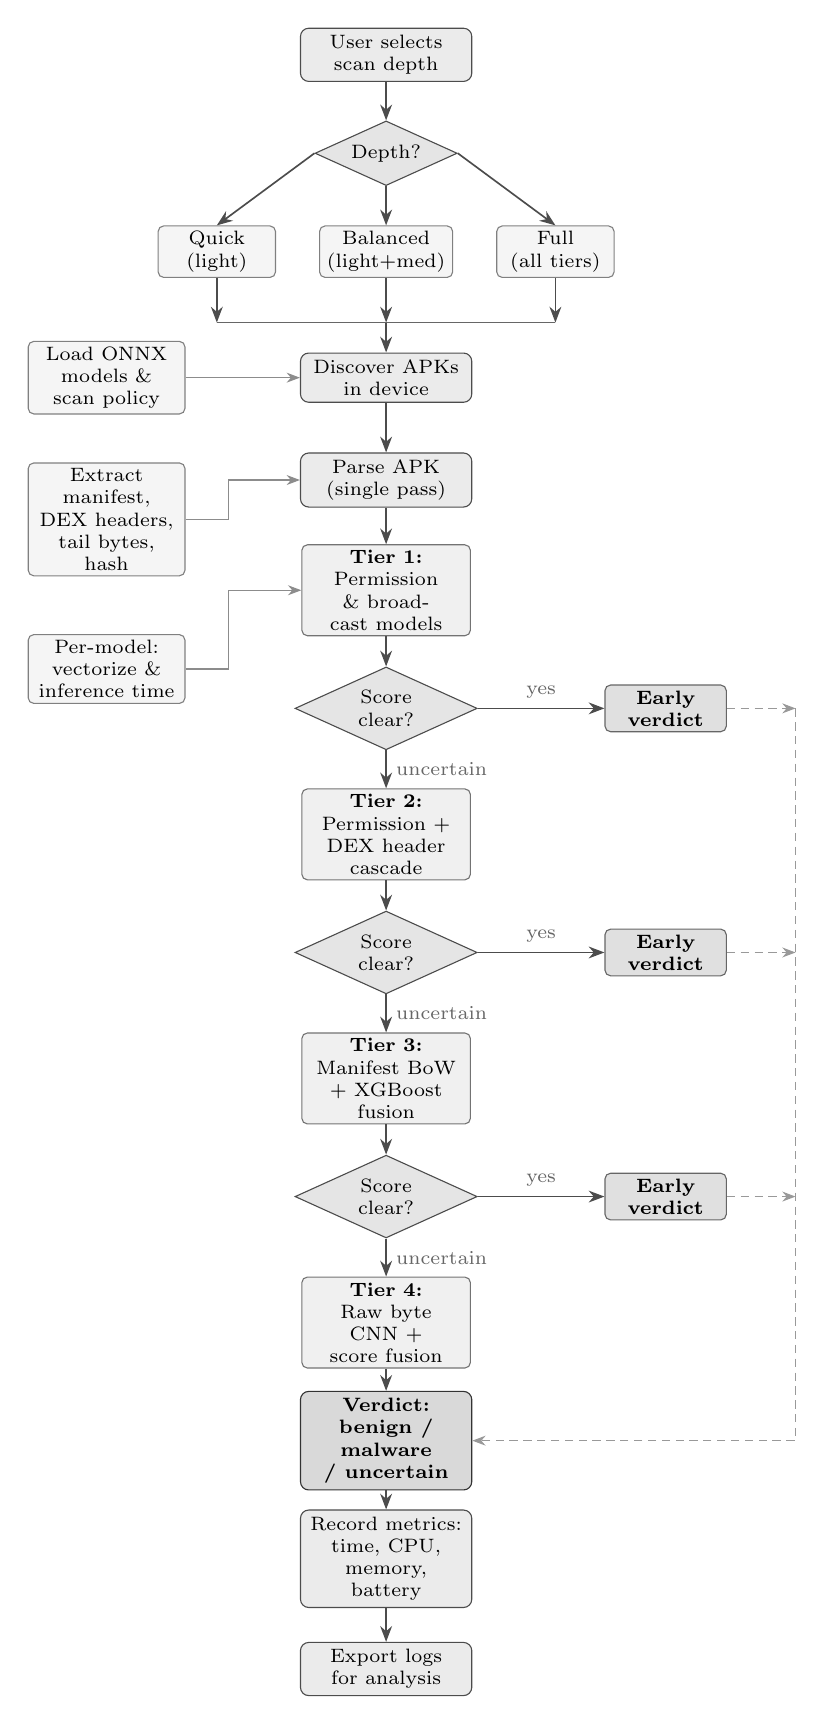
\begin{tikzpicture}[
  font=\scriptsize,
  >=Stealth,
  main/.style={
    rectangle, rounded corners=3pt,
    draw=black!70, fill=black!8,
    text width=2.0cm, align=center,
    minimum height=0.58cm, inner sep=2.5pt
  },
  decision/.style={
    diamond, aspect=2.2,
    draw=black!70, fill=black!10,
    text width=1.1cm, align=center,
    inner sep=1pt
  },
  verdict/.style={
    rectangle, rounded corners=3pt,
    draw=black!80, fill=black!15,
    text width=2.0cm, align=center,
    minimum height=0.55cm, inner sep=2.5pt,
    font=\scriptsize\bfseries
  },
  side/.style={
    rectangle, rounded corners=2pt,
    draw=black!50, fill=black!4,
    text width=1.85cm, align=center,
    minimum height=0.5cm, inner sep=2pt
  },
  tiernode/.style={
    rectangle, rounded corners=2pt,
    draw=black!55, fill=black!6,
    text width=2.0cm, align=center,
    minimum height=0.5cm, inner sep=2pt
  },
  exitnode/.style={
    rectangle, rounded corners=2pt,
    draw=black!60, fill=black!12,
    text width=1.4cm, align=center,
    minimum height=0.42cm, inner sep=2pt,
    font=\scriptsize\bfseries
  },
  arr/.style={->, semithick, black!70},
  sarr/.style={->, thin, black!45},
  darr/.style={->, densely dashed, thin, black!40},
  % CHANGED: label style now uses \scriptsize (normal) instead of \tiny\itshape
  lbl/.style={font=\scriptsize, black!60}
]

%% ── Top: user interaction ────────────────────────────────────────────
\node[main] (ui) at (0, 0.00) {User selects\\scan depth};
\node[decision] (depth) at (0,-1.25) {Depth?};

\node[side, text width=1.35cm] (dq) at (-2.15,-2.50) {Quick\\(light)};
\node[side, text width=1.55cm] (db) at ( 0.00,-2.50) {Balanced\\(light+med)};
\node[side, text width=1.35cm] (df) at ( 2.15,-2.50) {Full\\(all tiers)};

\draw[arr] (ui) -- (depth);
\draw[arr] (depth.west) -- (dq.north);
\draw[arr] (depth.south) -- (db.north);
\draw[arr] (depth.east) -- (df.north);

%% ── Merge to scan ───────────────────────────────────────────────────
\node[main] (scan) at (0,-4.10) {Discover APKs\\in device};
\draw[arr] (dq.south) -- (-2.15,-3.40);
\draw[arr] (db.south) -- ( 0.00,-3.40);
\draw[arr] (df.south) -- ( 2.15,-3.40);
\draw[black!60] (-2.15,-3.40) -- (2.15,-3.40);
\draw[arr] (0,-3.40) -- (scan.north);

%% ── Parse once ──────────────────────────────────────────────────────
\node[main] (parse) at (0,-5.40) {Parse APK\\(single pass)};
\draw[arr] (scan) -- (parse);

%% ── Tier 1 (defined early so annotations can reference it) ──────────
\node[tiernode] (t1) at (0,-6.80) {
  \textbf{Tier 1:} Permission\\
  \& broadcast models
};
\draw[arr] (parse) -- (t1);

%% ── Left annotations — staggered with gaps ──────────────────────────
\node[side] (rscan) at (-3.55,-4.10) {
  Load ONNX\\
  models \&\\
  scan policy
};
\draw[sarr] (rscan.east) -- (scan.west);

\node[side] (fctx) at (-3.55,-5.90) {
  Extract manifest,\\
  DEX headers,\\
  tail bytes, hash
};
\draw[sarr] (fctx.east) -- ++(0.55,0) |- (parse.west);

\node[side] (rmetric) at (-3.55,-7.80) {
  Per-model:\\
  vectorize \&\\
  inference time
};
\draw[sarr] (rmetric.east) -- ++(0.55,0) |- (t1.west);

%% ── Tier 1 decision — MORE vertical gap ─────────────────────────────
\node[decision] (d1) at (0,-8.30) {Score\\clear?};
\draw[arr] (t1) -- (d1);

\node[exitnode] (e1) at (3.55,-8.30) {Early\\verdict};
\draw[arr] (d1.east) -- node[above, lbl] {yes} (e1.west);

%% ── Tier 2 — increased gap from d1 ─────────────────────────────────
\node[tiernode] (t2) at (0,-9.90) {
  \textbf{Tier 2:} Permission +\\
  DEX header cascade
};
\draw[arr] (d1.south) -- node[right, lbl] {uncertain} (t2.north);

\node[decision] (d2) at (0,-11.40) {Score\\clear?};
\draw[arr] (t2) -- (d2);

\node[exitnode] (e2) at (3.55,-11.40) {Early\\verdict};
\draw[arr] (d2.east) -- node[above, lbl] {yes} (e2.west);

%% ── Tier 3 — increased gap from d2 ─────────────────────────────────
\node[tiernode] (t3) at (0,-13.00) {
  \textbf{Tier 3:} Manifest BoW\\
  + XGBoost fusion
};
\draw[arr] (d2.south) -- node[right, lbl] {uncertain} (t3.north);

\node[decision] (d3) at (0,-14.50) {Score\\clear?};
\draw[arr] (t3) -- (d3);

\node[exitnode] (e3) at (3.55,-14.50) {Early\\verdict};
\draw[arr] (d3.east) -- node[above, lbl] {yes} (e3.west);

%% ── Tier 4 — increased gap from d3 ─────────────────────────────────
\node[tiernode] (t4) at (0,-16.10) {
  \textbf{Tier 4:} Raw byte\\
  CNN + score fusion
};
\draw[arr] (d3.south) -- node[right, lbl] {uncertain} (t4.north);

%% ── Final verdict ───────────────────────────────────────────────────
\node[verdict] (verd) at (0,-17.60) {
  Verdict:\\
  benign / malware\\
  / uncertain
};
\draw[arr] (t4) -- (verd);

%% ── Early-exit dashed arrows — far-right corridor at x=5.20 ────────
\draw[darr] (e1.east) -- (5.20,-8.30);
\draw[darr] (e2.east) -- (5.20,-11.40);
\draw[darr] (e3.east) -- (5.20,-14.50);
\draw[darr] (5.20,-8.30) -- (5.20,-17.60) -- (verd.east);

%% ── Metrics logging ────────────────────────────────────────────────
\node[main] (log) at (0,-19.10) {
  Record metrics:\\
  time, CPU,\\
  memory, battery
};
\draw[arr] (verd) -- (log);

\node[main] (export) at (0,-20.50) {
  Export logs\\
  for analysis
};
\draw[arr] (log) -- (export);

\end{tikzpicture}%
}

\vspace{4pt}
\noindent\scriptsize\textbf{Fig.\,2.} VigiDroid on-device scanning flow.
The app parses each APK once, then runs a tiered cascade of increasingly
expensive models---exiting early when a confident score is reached---and
logs per-stage resource metrics for thesis evaluation.

\end{document}
